% \begin{savequote}[8cm]
% Alles Gescheite ist schon gedacht worden.\\
% Man muss nur versuchen, es noch einmal zu denken.

% All intelligent thoughts have already been thought;\\
% what is necessary is only to try to think them again.
%   \qauthor{--- Johann Wolfgang von Goethe \cite{von_goethe_wilhelm_1829}}
% \end{savequote}

\chapter{\label{ch:2-neutrinophysics}Neutrino physics}

\minitoc

This chapter includes a brief historical overview and a review of the introductory theoretical background of neutrino physics. In particular, the mechanism of neutrino oscillations will be described and several neutrino experimental anomalies will be analyzed. The constraints and the hints for additional, non-weakly interacting neutrino states, will also be presented.

\section{Introduction}

Neutrino physics represents one of the most exciting areas of active research in particle physics. The history of the early days of particle physics shows that neutrinos have challenged physicists since the famous Pauli's letter to his fellow \emph{Radioactive Ladies and Gentlemen} \cite{Pauli:1930pc}. The continuous spectrum of the nuclear $\beta$-decay was then hypothesized by Fermi to be caused by the three-body process:
\begin{equation}
    n\rightarrow p + e^{-} + \bar{\nu}_{e},
\end{equation}
and mediated by a four-fermion interaction in the form of:
\begin{equation}
    \frac{G_{F}}{\sqrt{2}}(\bar{n}\Gamma_{N}p)(\bar{\nu}_{e}\Gamma_{L}e),
\end{equation}
where, in modern terms, $G_{F}$ is the Fermi constant and $\Gamma_{N,L}$ are a linear combination of the \emph{gamma matrices}. The Feynman diagram of the four-fermion approximation of $\beta$-decay is shown in Figure \ref{fig:fermibeta}.

\begin{figure}
    \centering
    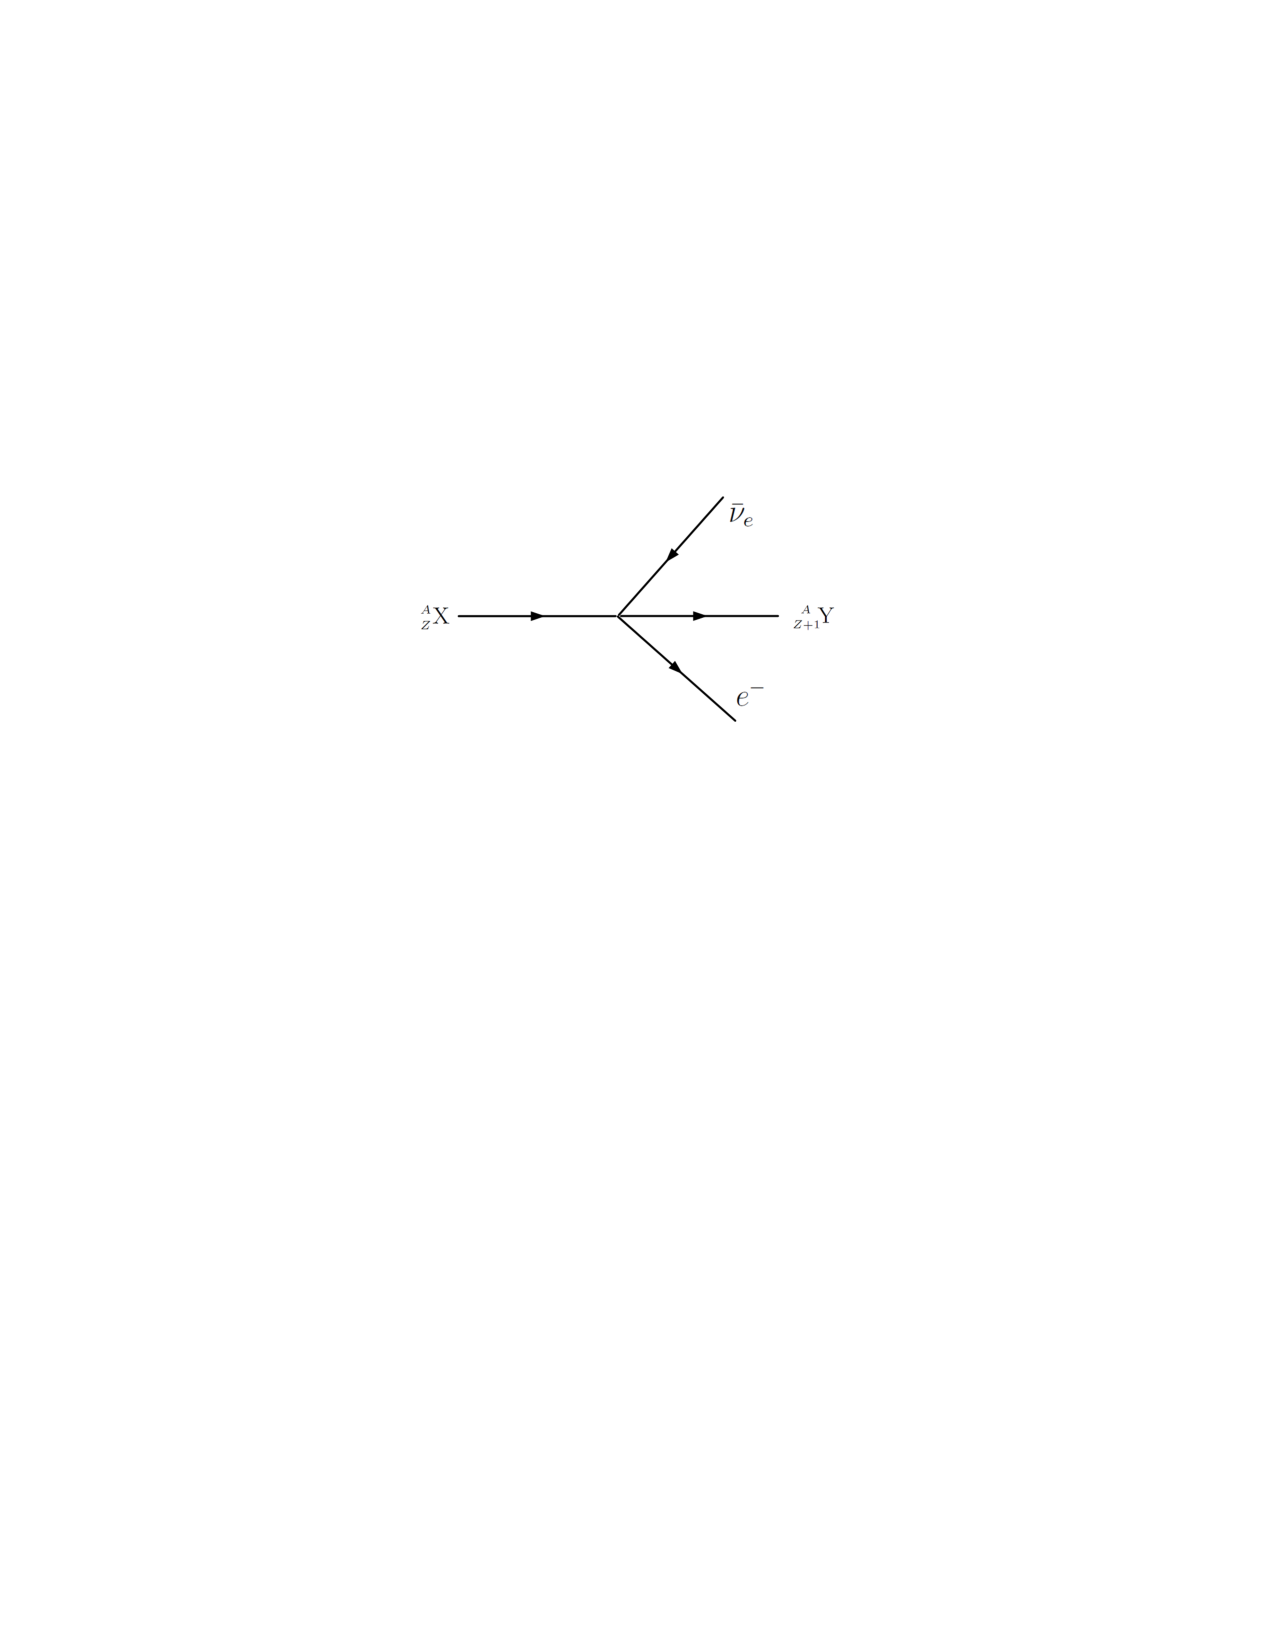
\includegraphics{figures/fermidecay.pdf}
    \caption{Feynman diagram of the $\beta$-decay of a $^{A}_{Z}X$ into a $^{A}_{Z+1}Y$ nucleus in the Fermi approximation.}
    \label{fig:fermibeta}
\end{figure}

This theory paved the way for the first experimental direct detection of neutrinos by Cowan and Reines in 1956 \cite{Cowan:1992xc}, which exploited the inverse $\beta$-decay process:
\begin{equation}
    \bar{\nu}_{e} + p \rightarrow e^{+} + n.
\end{equation}
The key detection technique, still used in modern reactor experiments, employed the detection of the $e^{+}e^{-}\rightarrow 2\gamma$ annihilation and a the $\gamma$ emitted by the recoiling neutron shortly afterwards. 

The leptonic current $\bar{\nu}_{e}\Gamma_{L}e$ was later verified to be left-handed in the form of $\gamma_{\mu}(1-\gamma_{5})$ ($V-A$). 
For massless neutrinos this allows to assign a left-handed (right-handed) helicity to neutrinos (anti-neutrinos), which was experimentally verified by Goldhaber in 1958 \cite{Goldhaber:1958nb}.

\section{Neutrino Oscillations}
In the modern Standard Model of particle physics there are three flavours of (anti)neutrinos ($\nu_{e}$, $\nu_{\mu}$, $\nu_{\tau}$), each one paired to a charged (anti)lepton ($e$, $\mu$, $\tau$ respectively). 
However, if neutrinos have masses, it is possible to have three (or more) neutrino mass eigenstates ($\nu_{1}$, $\nu_{2}$, $\nu_{3}$, ...) analogues of the charged-lepton mass eigenstates. 
In this case, a neutrino produced as a flavour eigenstate would \emph{oscillate} through its path and change to another flavor eigenstate. This happens because the flavour eigenstate is a mixture of the three (or more) mass eigenstates, which travel with different wavelengths and create interference patterns. 

The oscillation probabilities can be easily derived in the case of two neutrino generations, which we follow for didactic reasons largely following the approach in \cite{deGouvea:2004gd}. The flavour eigenstates $\nu_{\alpha}, \nu_{\beta}$ can be expressed as a superposition of the two mass eigenstates $\nu_1$ and $\nu_2$ using the nominal rotation matrix $U$:
\begin{equation}
U = \begin{bmatrix}
    \cos\theta & -\sin\theta \\
    \cos\theta & \sin\theta
    \end{bmatrix}.
\end{equation}

The flavour neutrino $\nu_{\alpha}$ will then propagate as: 
\begin{equation}
    \key{\nu_{\alpha}} = \cos\theta\ket{\nu_{1}}+\sin\theta\ket{\nu_{2}}
\end{equation}